\begin{apendicesenv}

% \partapendices

\chapter{Estrutura do Portifólio Tecnológico}
\begin{itemize}
\item Apresentação
\item Características
\item Dicas
\item Especialistas
\item Instalação
\item Pré-requisitos
\item Recomendações de uso
\item Referências Bibliográficas
\item Links para sites e páginas que tratam do assunto na Web
\item Experiências ocorridas na empresa (Problemas e Soluções)
\end{itemize}

\chapter{Exemplo de Questionário de Satisfação de Cliente}
Questionário   criado   com   base   no   “Modelo   de   Satisfação   de   Clientes”   do   site   SurveyMonkey  
[ SURVEY ].  

1. Quão profissional é a nossa empresa? \\
( ) Extremamente profissional \\
( ) Muito profissional \\
( ) Moderadamente profissional \\
( ) Pouco profissional \\
( ) Nada profissional \\

2. Em comparação com os nossos competidores, a qualidade do nosso serviço é superior, inferior ou a 
mesma? \\
( ) Extremamente superior \\
( ) Moderadamente superior \\
( ) Mesma \\
( ) Moderadamente inferior \\
( ) Extremamente inferior \\
 
3. Em comparação com os nossos competidores, o preço do nosso serviço é superior, inferior, ou o 
mesmo? \\
( ) Muito superior \\
( ) Pouco superior \\
( ) Mesma \\
( ) Pouco inferior \\
( ) Muito inferior \\
 
4. Quão prestativa é a nossa empresa? ( ) Extremamente prestativa \\
( ) Muito prestativa \\
( ) Moderadamente prestativa \\
( ) Pouco prestativa \\
( ) Nada prestativa \\
 
5.  De forma geral, quão satisfeito ou insatisfeito está com os colaboradores da nossa empresa? \\
( ) Muito satisfeito \\
( ) Pouco satisfeito \\
( ) Nem satisfeito nem insatisfeito \\
( ) Pouco insatisfeito \\
( ) Muito insatisfeito \\
 
6. Gosta da nossa empresa, não gosta nem detesta, ou detesta? \\
( ) Gosto muito \\
( ) Gosto pouco \\
( ) Não gosto nem detesto \\
( ) Detesto pouco \\
( ) Detesto muito \\
 
7. Gosta da nossa empresa, não gosta nem detesta, ou detesta? \\
( ) Extremamente provável \\
( ) Muito provável \\
( ) Moderadamente provável \\
( ) Pouco provável( ) Nada provável\\


\chapter{Protótipo do Repositório de Conhecimento}

\begin{figure}[H]
\centering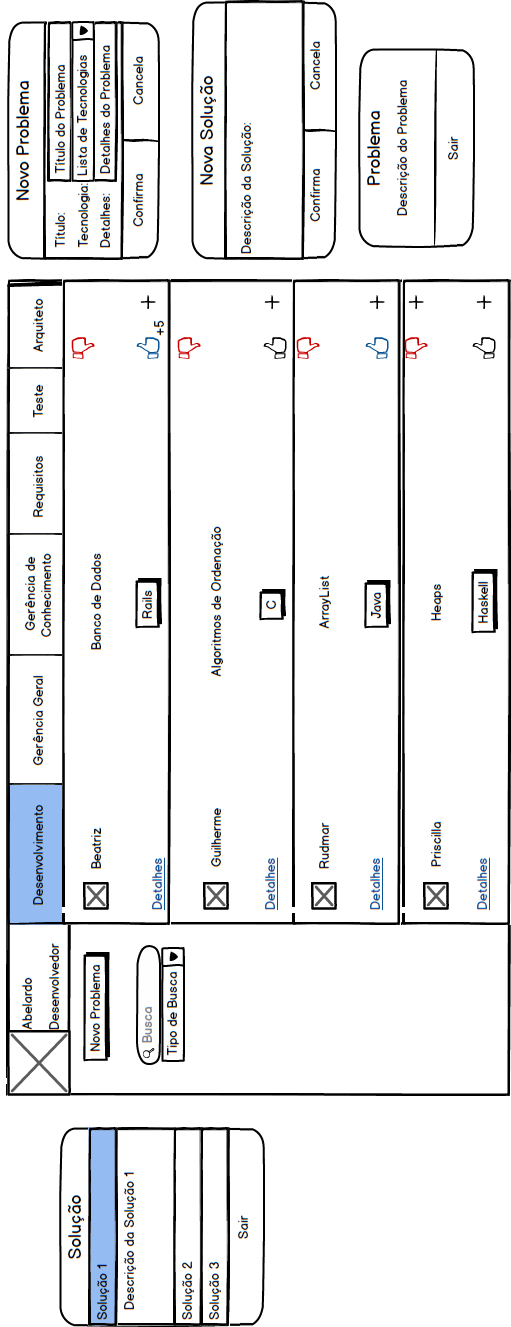
\includegraphics[scale=0.5]{figuras/prototipo.png}
\caption{\textit{Protótipo do Repositório de Conhecimento}}
\end{figure}

\chapter{Cronograma}

\begin{figure}[H]
\centering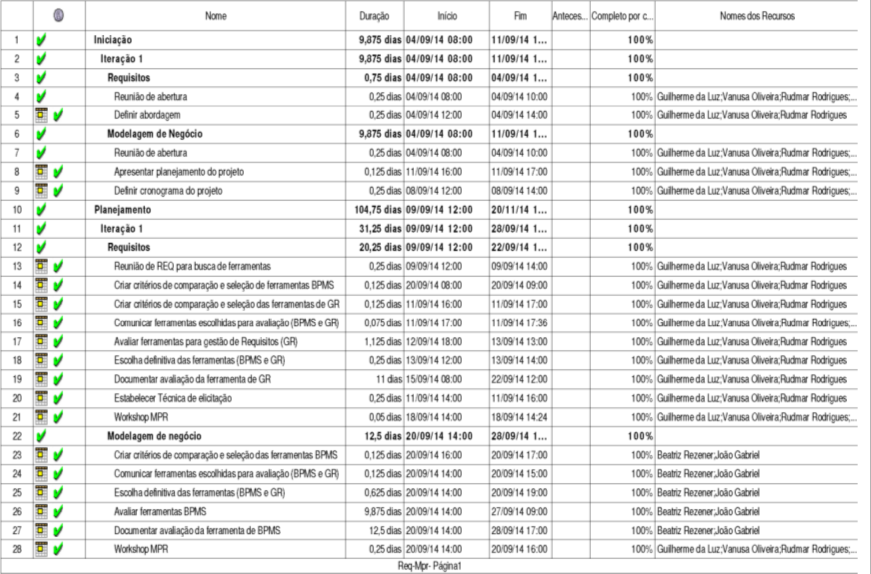
\includegraphics[scale=0.5]{figuras/cronograma1.pdf}
\caption{\textit{Página 1 do Cronograma}}
\end{figure}

\begin{figure}[H]
\centering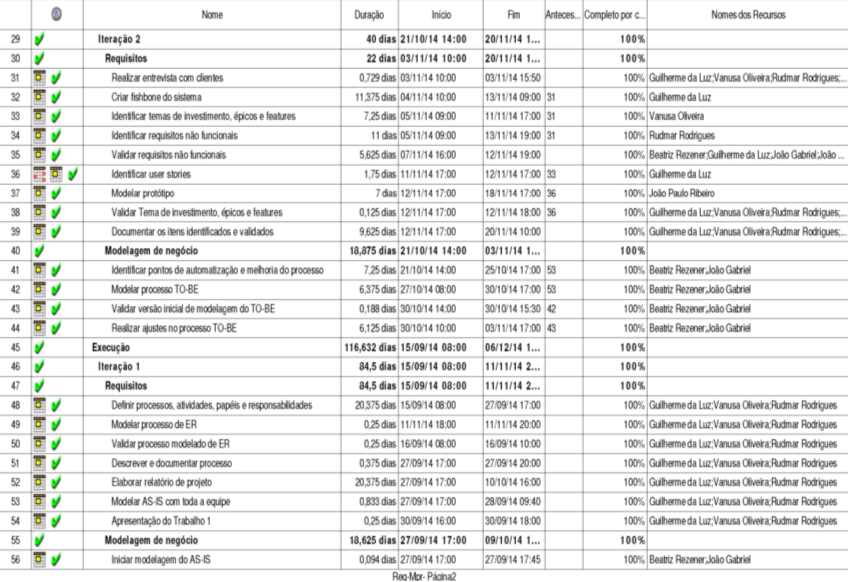
\includegraphics[scale=0.5]{figuras/cronograma2.pdf}
\caption{\textit{Página 2 do Cronograma}}
\end{figure}

\begin{figure}[H]
\centering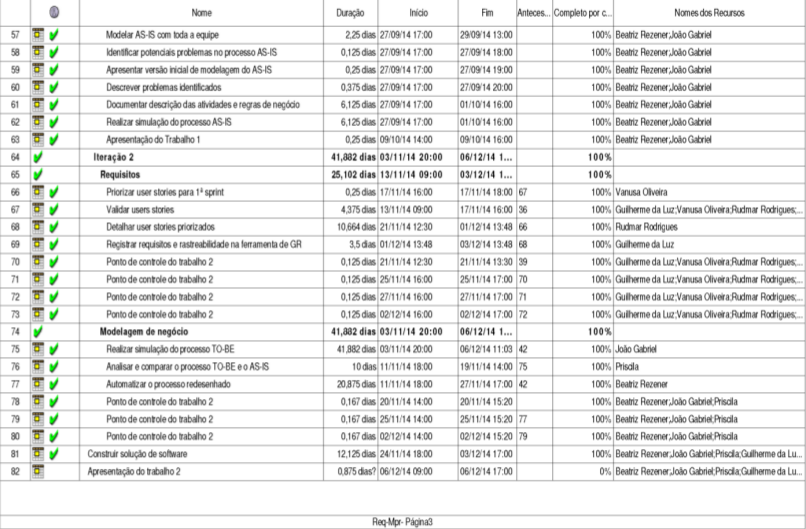
\includegraphics[scale=0.5]{figuras/cronograma3.pdf}
\caption{\textit{Página 3 do Cronograma}}
\end{figure}

\chapter{Processos de ER}

\begin{figure}[H]
\centering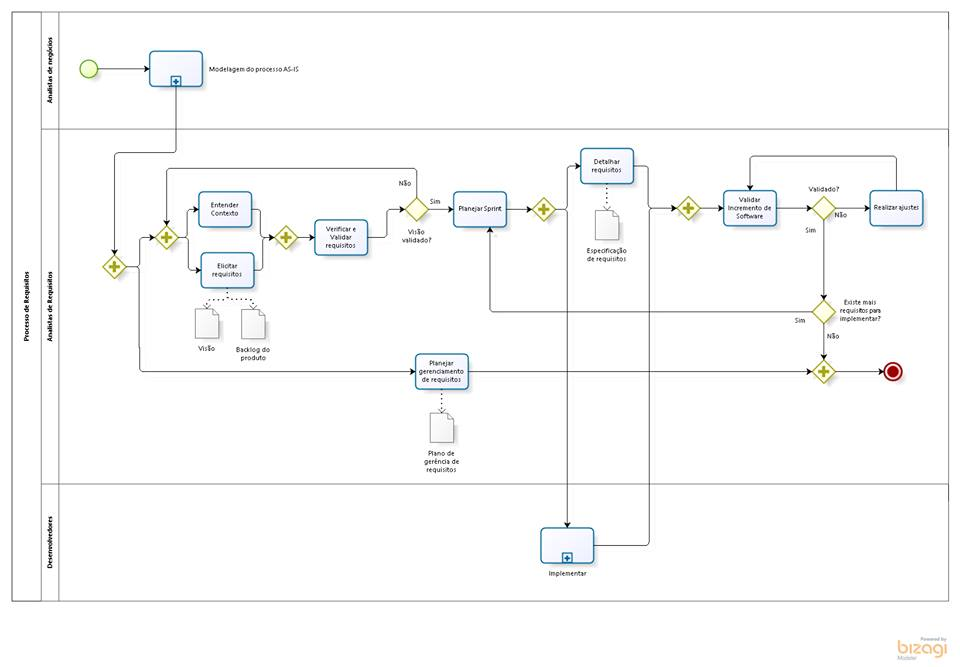
\includegraphics[scale=0.5]{figuras/processoAntigo}
\caption{\textit{Processo Antigo de ER}}
\end{figure}

\begin{figure}[H]
\centering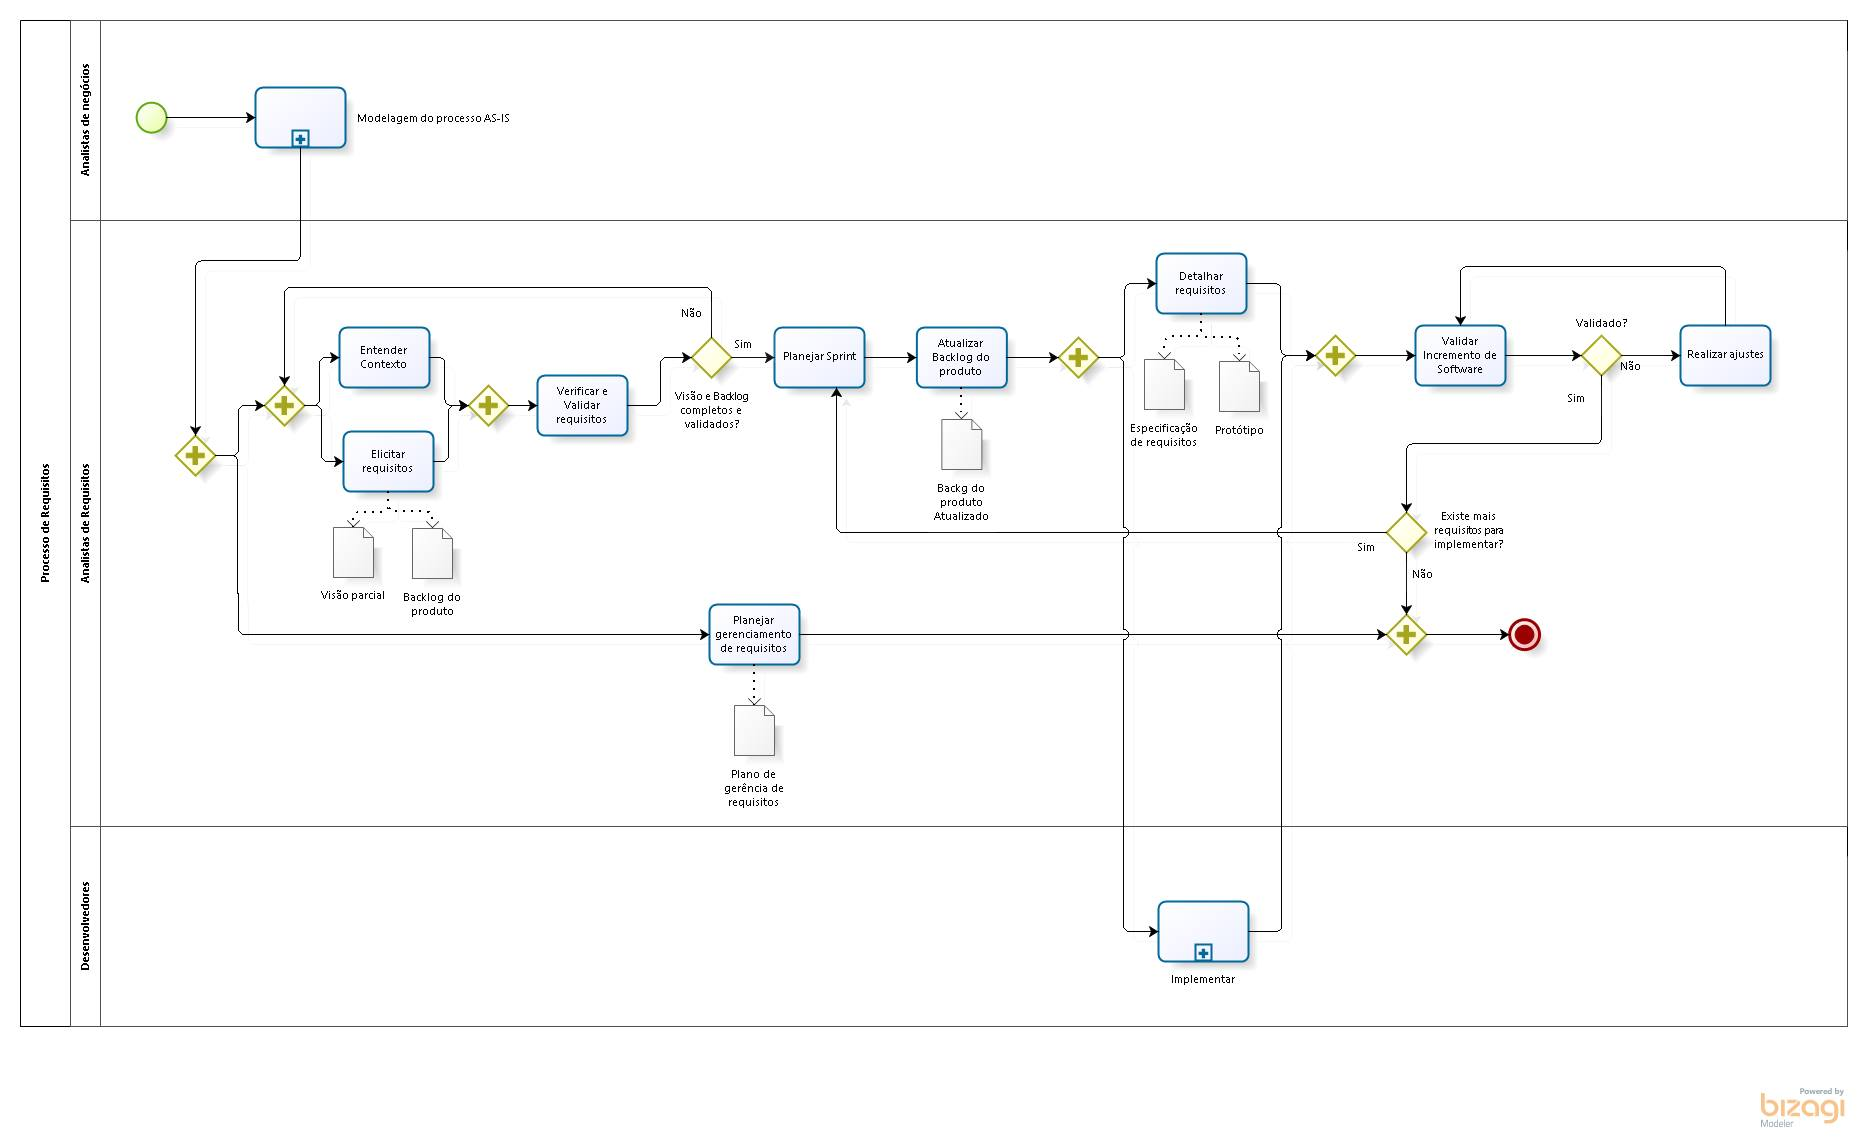
\includegraphics[scale=0.3]{figuras/processoAtual}
\caption{\textit{Processo Atual de ER}}
\end{figure}

\end{apendicesenv}
